%*****************************************************************************************************            
%                               INSTITUT MINES-TELECOM, IMT ATlantique
%                         Département Mathematical & Electrical Engineering           
%                                     Technopôle de Brest-Iroise                   
%                                  CS 83818 - 29238 BREST Cedex 3                       
%            
%                                    **  Tous droits réservés **
%                                      
%
% NOM DU PROJET : TP LaTeX 006 / Modèle de rapport de recherche (validé par la DRI), de support de cours
% et de TP au format LaTeX avec les éléments de la charte graphique de la communication d'IMT Atlantique
%
% LIVRABLE : [ ] Memo, [ ] Résumé, [ ] Article, [ ] Code, [X] Rapport , [ ] Thèse, [ ] Cours/TP
%
% AUTEUR(s) : Thierry LE GALL (Dépt. MEE), Guillaume ANSEL (SC), Thomas GUILMENT (Dépt. SC)
%
% 
%***********************************************************************************************

%-----------------------------------------------------------------------------------------------
%                                    DEBUT DU FICHIER D'EDITION
%-----------------------------------------------------------------------------------------------

\documentclass[11pt,a4paper,french]{article}

\usepackage{babel}
\usepackage[utf8]{inputenc}
\usepackage[T1]{fontenc}

\usepackage{newtxtext} % Police pour texte
\usepackage{newtxmath} % Police pour formules
\usepackage{textcomp}
\usepackage{graphicx}
\usepackage{amsmath}
\usepackage{microtype}
\usepackage{amsmath}
\usepackage[
    left = \flqq{},% 
    right = \frqq{},% 
    leftsub = \flq{},% 
    rightsub = \frq{} %
]{dirtytalk}
\usepackage{nicefrac}
\usepackage{multirow}
\usepackage{enumitem}
\usepackage{framed}	% Permet de surligner les résultats importants

% Charte graphique de IMT Atlantique
% L'option "version" affiche la menion "Document version x" sur la première de couverture
% Le numéro de version est paramétrable via la commande "\version"
% L'option "copyright" affiche la mention "© IMT Atlantique ..." sur la quatrième de couverture
% Les informations de copyright sont paramétrables via les commandes \IMTAanneecopyright, \IMTAdepotlegal, \IMTAissn

\usepackage[copyright]{../sty/imta} % édition avec copyright (et n°ISSN) en 4eme de couverture
%\usepackage{../sty/imta}	% édition sans copyright (et n°ISSN) en 4eme de couverture

% Signets et hyperliens (à charger en dernier)
\usepackage[colorlinks=true,linkcolor=black,urlcolor=blue,citecolor=IMTAbleu]{hyperref} 

%----------------- Métadonnées du PDF (facilite le travail des moteurs de recherche) -----------
\hypersetup{
	pdfinfo = {
		Author = {SANTOS SEISDEDOS, Carlos},
		Title = {TP Sens Électrique},
		Keywords = {Sens Électrique; Robotique Bio-Inspirée; ...}
	}
}

%--------------------------- Définition du contenu du pied de page ----------------------------

% Le pied de page contient par défaut le titre du document.
% Il peut être remplacé en décommentant l'une des lignes ci-dessous

%\IMTAfooter{Modèle de document \LaTeX{} IMT Atlantique} % Exemple de remplacement par un autre texte
\IMTAfooter{\thereportnumber} % Utilisation du numéro de rapport de recherche

%-------------------- Informations de copyright pour quatrième de couverture ------------------
%          (uniquement si l'option "copyright" est présente pour le package imta)

% Les lignes ci-dessous permettent de remplacer manuellement le mois et l'année
% d'édition pour le dépot légal si nécessaire. Par défaut, le mois et l'année
% courants lors de la compilation du document sont utilisés

\IMTAanneecopyright{2021}
\IMTAdepotlegal{Septembre 2017}

%-------------------------------------- Do not modify -----------------------------------------
																									
% le numéro ISSN est communiqué par la BNF à la DRI. N°fixé par la BNF en
% fonction du type de document. Ne concerne que la collection des rapports
% de recherche (et pas les autres types de document utilisant ce modèle).
\IMTAissn{2556-5060}

%----------------------------------- End of do not modify -------------------------------------

%----------------- Définitions d'ensembles et d'opérateurs mathématiques ----------------------

\def\Cset{\mathbb{C}} % complexes
\def\Hset{\mathbb{H}} % hilbert
\def\Nset{\mathbb{N}} % entiers naturels
\def\Qset{\mathbb{Q}} % rationnels
\def\Rset{\mathbb{R}} % reels
\def\Zset{\mathbb{Z}} % entiers relatifs
\def\Dset{\mathbb{D}} % disque unite ouvert
\def\Eset{\mathbb{E}} % esperance mathematique

%-------------------------------------- FIN DES DEFINITIONS ----------------------------------

\begin{document}

%---------------------------------------------------------------------------------------------
%                                   PAGE DE TITRE (please modify)
%---------------------------------------------------------------------------------------------

% Type de document
%\DocumentType{<Type de document>}  
%\DocumentType{Collection des rapports de recherche d'IMT Atlantique}
%\DocumentType{Document support de BE et de TP}
%\DocumentType{Support de cours}
\DocumentType{\Large{TP - Sens Électrique}}
%\DocumentType{Mémoire technique}


% Numéro de rapport de recherche (à remplacer)
% Commenter la ligne ci-dessous si le document n'est pas un rapport de recherche
%\ReportNumber{N° rapport de recherche}


\entity{%\textbf{\large{IMT Atlantique}}\\
% Dépt. Automatique productique et informatique\\
% Dépt. Électronique\\ 
% Dépt. Informatique\\ 
%Dépt. Image \& traitement de l'information\\
%Dépt. Langues \& culture internationale\\ 
%Dépt. Logique des usages, sciences sociales \& sciences de l'information\\ 
%Dépt. Micro-ondes\\ 
%Dépt. Optique\\
%Dépt. Physiques subatomiques et technologies\\
%Dépt. Sciences sociales et de gestion\\
%Dépt. Mathematical \& Electrical Engineering\\
%Dépt. Systèmes énergétiques et environnement\\
%Dépt. Systèmes réseaux, cybersécurité et droit du numérique\\
%Technopôle de Brest-Iroise - CS 83818\\
%29238 Brest Cedex 3\\
%Téléphone: +33 (0)2 29 00 13 04\\
%Télécopie: +33 (0)2 29 00 10 12\\
%4, rue Alfred Kastler\\
%CS 20722\\
%44307 Nantes Cedex 3\\
%Téléphone: +33 (0)2 51 85 81 00\\
%Télécopie: +33 (0)2 99 12 70 08\\		
%2, rue de la Châtaigneraie\\
%CS 17607\\
%35576 Cesson Sévigné Cedex\\
%Téléphone: +33 (0)2 99 12 70 00\\
%Télécopie: +33 (0)2 51 85 81 99\\
%10, avenue Édouard Belin\\
%BP 44004\\
%31028 Toulouse Cedex 04\\
%Téléphone: +33 (0)5 61 33 83 65\\		
%URL: \textbf{\href{http://www.imt-atlantique.fr/}{www.imt-atlantique.fr}}
}

%\docdescription{<Destinataire : >}

\title{Robotique Bio Inspirée (ROBIO)}
%\title{Étude d'une forme d'onde pour communications longues-distances par le canal acoustique sous-marin}

\author{Carlos SANTOS SEISDEDOS}

% Numéro de version du document, affiché sur la couverture
% Commenter cette ligne pour ne pas faire apparaître la version du document.
\version{2.0}

% Date d'édition du document
\date{\today}

%------------------------------------------ Do not modify ------------------------------------
\IMTAfrontcover
\pagestyle{IMTAfancy} % Changement du style de page pour avoir en-tête et pied de page
%--------------------------------------- End of do not modify --------------------------------

%% Affichage des listes et tables.
\IMTAsommaire
\newpage
\IMTAlistefigures  % commenter pour ne pas avoir la liste des figures
\IMTAlistetableaux   % commenter pour ne pas avoir la liste des tables
\newpage
%---------------------------------------------------------------------------------------------
%                                   INTRODUCTION (please modify)
%---------------------------------------------------------------------------------------------

\section{Introduction}

La perception active est basée sur l'émission d'un champ électrique de nature dipolaire qui s'oriente le plus souvent horizontalement le long de leur corps. \cite{BENACHENHOU2014}
\section{Démarche de Modélisation}
\subsection{Le robot poisson}

Le robot (robot poisson ou poisson) simulé est composé de 5 électrodes pour faire de l'\textit{électrolocation active}, c'est-à-dire pour générer un champ électrique qui réagit à l'environnement, tout comme le \textit{Gnathonemus petersii}. La suivante figure en deux dimension (le 5-ième capteur n'est pas représenté) montre le robot poisson simulé, ainsi que l'emplacement des électrodes. 

\begin{figure}[h!]
    \centering
    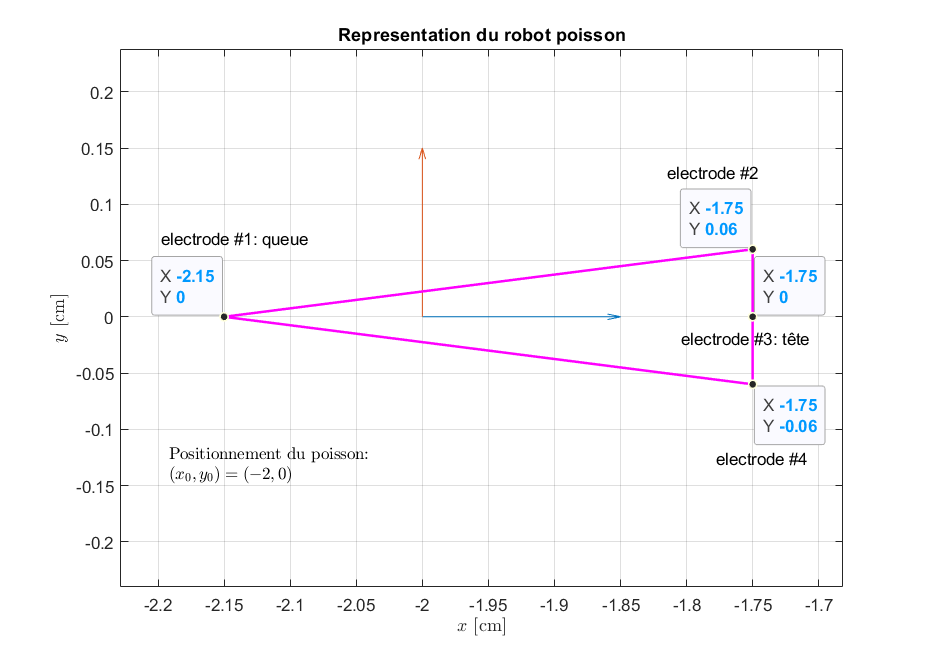
\includegraphics[width=\textwidth]{assets/poisson/poisson.png}
    \caption{Représentation du robot poisson et des capteurs dans le simulateur MATLAB}
    \label{fig:poisson}
\end{figure}

\subsection{La méthode des réflexions}
La méthode des réflexions est une solution au problème d'électrolocation directe, présentée sur \cite{Boyer2012}. Cette technique consiste à résoudre l'équation de Laplace $\Delta\phi = 0$ dans un scénario avec plusieurs objets autour du capteur et avec certaines conditions imposées aux objets (capteur inclus). En appliquant le principe de superposition présenté, nous pouvons résoudre l'équation de Laplace en considérant seulement les deux premières réflexions dans l'environnement du capteur et négligeant le reste des réflexions: nous tenons en compte donc l'émission du capteur $\phi_0$ en absence de tout objet, la réflexion de ce potentiel sur un objet et la seconde réflexion du potentiel émis par l'objet sur le capteur. La Figure \ref{fig:reflexions} résume bien le principe de cette méthode itérative. Chaque potentiel $\phi_i$ représente la réponse à la somme des potentiels $\phi_0 + \phi_1 + \dots \phi_{i-1}$ réfléchis par les objets qui entourent le capteur, et le capteur. Par conséquent, le problème se réduit à trouver les courants associés au potentiel de base $\phi_0$, la première et la seconde réflexion: $I^{(0)}, I^{(1)}$ et $I^{(2)}$. 
\clearpage 
\begin{figure}[h!]
    \centering
    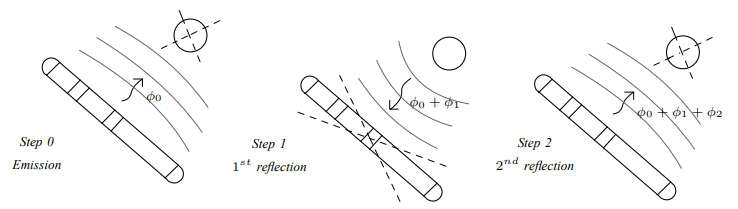
\includegraphics[width=0.8\textwidth]{doc/img/reflexions.png}
    \caption{Schéma des trois premières réflexions de la Méthode des Réflexions, image de \cite{Boyer2012}}
    \label{fig:reflexions}
\end{figure}

Le courant $I^{(0)}$ représente uniquement l'émetteur, il peut être obtenu en utilisant un simulateur numérique et s'écrit: 

\begin{equation}
    I^{(0)} = \bar{C}^{(0)} \cdot U
\end{equation}

avec $U$ étant le vecteur tension, dans notre cas $U = \left [1, 0, 0, 0, 0 \right ]$ car seulement l'électrode à la queue est alimenté, et $\bar{C}^{(0)}$ étant la matrice de conductances à vide entre chaque électrode et ayant la suivante forme dans notre cas: 
\begin{center}
$\bar{C}^{(0)} = \gamma \cdot 
\begin{pmatrix}
0.2557 & -0.0639 & -0.0639 & -0.0639 & -0.063 \\
-0.0639 & 0.1218 & -0.0203 & -0.0173 & -0.0203 \\
-0.0639 & -0.0203 & 0.1218 & -0.0203 & -0.0173 \\
-0.0639 & -0.0173 & -0.0203 & 0.1218 & -0.0203 \\
-0.0639 & -0.0203 & -0.0173 & -0.0203 & 0.1218 \\
\end{pmatrix}$
\end{center}

avec $\gamma$ la conductivité de l'eau $\left ( \text{en } \frac{S}{cm} \right )$.

Les courants $I^{(1)}$ et $I^{(2)}$ doivent être calculés en temps réel car ils dépendent de la position du capteur et du reste des objets. Nous divisons le courant généré par les réflexions en une composante axiale et une composante latérale. D'après \cite{Boyer2012}, \say{ la composante axiale $I_{\text{ax}}$ traduit la réaction du capteur aux différences de potentiel réfléchies par l'objet et évaluées le long de l'axe du capteur, et la composante latérale $I_{\text{lat}}$ traduit la polarisation latérale du capteur générée par le flux latéral du champ renvoyé par l'objet }: 

\begin{equation}
    I = I_{\text{ax}} + I_{\text{lat}}
\end{equation}
avec
\begin{equation}
    I_{\text{ax}} = \left ( 1- \bar{C}^{(0)} \cdot K \right ) \cdot P_{+} \cdot I^{(0)}
\end{equation}
et 
\begin{equation}
    I_{\text{lat}} = P_{\perp} \cdot L \cdot P_{+} \cdot I^{(0)}
\end{equation}

où, la matrice $P_{+}$ projette les courants à travers chaque électrode, en additionnant les courants de la même électrode, la matrice diagonale $P_{\perp}$ dépend de la géométrie du capteur, et les matrices $K$ et $L$ dépendent de la géométrie de l'objet et de sa position et orientation par rapport au capteur. 

Afin de simplifier le simulateur, nous allons négliger le courant latérale. En remplaçant le courant de base, le courant à étudier pour le contrôle du robot est de la forme: 

\begin{equation}
    I= \bar{C}^{(0)} \cdot U \left ( 1- \bar{C}^{(0)} \cdot K \right )
\end{equation}

Dans ce qui suit, nous devons calculer la matrice $K$ pour les différents objets que le capteur peut rencontrer. Nous allons considérer uniquement le cas d'un petit objet qui peut être isolant ou conducteur, et le cas d'un mur isolant. Notre simulateur placera des objets dans l'aquarium composé de 4 murs isolants. 
\newpage
\subsubsection{Cas d'un petit objet}
Pour le calcul de la matrice $K$ dans le cas d'un petit objet, nous prenons en compte le scénario composé d'un capteur (ou une électrode $\varepsilon_{\alpha}$), qui a pour centre $x_\alpha$, et d'un petit objet $\mathbf{p}$, qui lui a pour centre $y_c$.
\begin{figure}[h!]
    \centering
    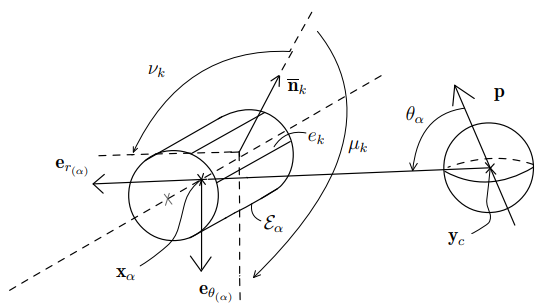
\includegraphics{doc/img/schema_petit_objet.png}
    \caption{Schéma représentant la macro-électrode $\varepsilon_{\alpha}$ du capteur perturbée par une sphère $\mathbf{p}$.}
    \label{fig:schema_petit_objet}
\end{figure}
Il est prouvé dans \cite{Boyer2012} que la matrice $K$ de réponse à cet objet suit l'expression suivante: 
\begin{equation}
    K = - \frac{1}{4\pi \cdot \gamma} \cdot \frac{r_\alpha \cdot P_r \cdot r_\beta}{\lVert r_\alpha \rVert^3 \cdot \lVert r_\beta \rVert^3}
\end{equation}
où, $r_\alpha = y_c - x_\alpha$, c'est-à-dire la distance entre l'objet et le capteur considéré, $r_\beta = y_c - x_\beta$, c'est-à-dire la distance entre l'objet et un autre capteur, et $P$ le tenseur de polarisation qui dépend de la géométrie de l'objet et du caractère conducteur/isolant. Pour une sphère, $P = \upchi \cdot a^3 \cdot I_{3}$ avec $I_3$ la matrice identité de $3$ dimensions, $a$ le rayon de la sphère et $\upchi$ le facteur de contraste: $1$ pour un objet totalement conducteur et $-0.5$ pour un objet totalement isolant.

Lors de la révision des résultats, vous trouverez la forme des courants lorsque le robot poisson traverse un objet totalement isolant et un objet totalement conducteur. 

\subsubsection{Cas d'un mur isolant}

Pour le cas des murs, nous utilisons la méthode présenté dans \cite{Jackson2012} pour des objets de grande taille. Comme illustré dans la Figure \ref{fig:schema_murs_coins}, cette méthode consiste à créer une image virtuelle du robot placée symétriquement au mur, qui a pour centre $x_\beta^*$ et, dans le cas d'approximation à un coin, une troisième image placée symétriquement au coin $C$. 

\begin{figure}[h!]
    \centering
    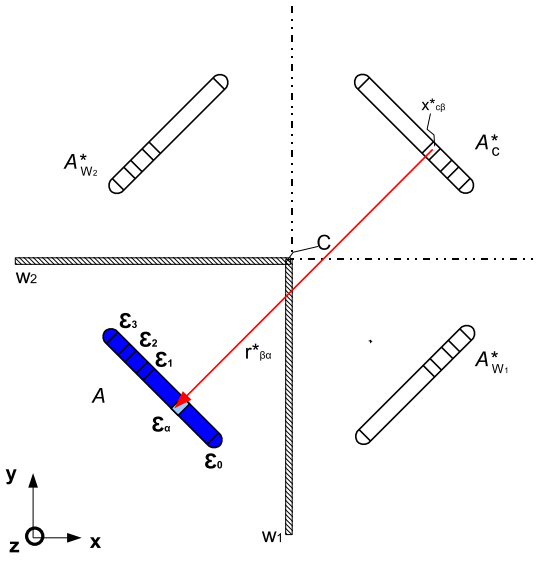
\includegraphics[scale=0.5]{doc/img/schema_murs_coins.png}
    \caption{Schéma représentant le capteur $A$ et les images virtuelles $A_{W_1}^*$ et $A_{W_2}^*$ symétriques aux murs $W_{1}$ et $W_{2}$, respectivement, et l'image virtuelle $A_C^*$ symétrique par rapport au coin $C$. }
    \label{fig:schema_murs_coins}
\end{figure}

En considérant le potentiel généré par le mur comme la superposition du champ du robot et le champ de son image, nous obtenons la matrice $K$ de réponse aux murs suivante: 

\begin{equation}
    K = - \frac{1}{4\pi \cdot \gamma} \cdot \frac{1}{\lVert r_{\beta\alpha}^* \rVert^3}
\end{equation}

où, $r_{\beta\alpha}^* = x_\alpha - x_\beta^*$ pour chaque combinaison d'électrode réel et électrode image. Du fait que notre aquarium porte 4 murs, nous avons 8 réflexions au total (4 réflexions provenant des murs et 4 réflexions provenant des coins). Dans la Figure \ref{fig:wall_reflexion} nous pouvons voir une représentation des 8 images virtuelles du robot poisson par rapport aux murs et aux coins. 

\begin{figure}
    \centering
    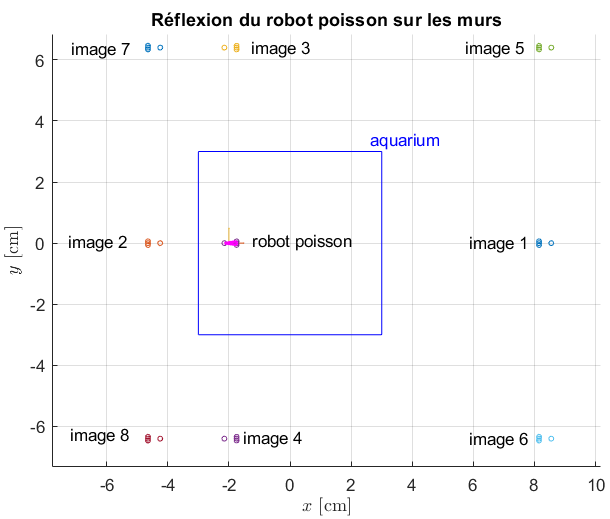
\includegraphics[scale=0.8]{assets/wall_reflexions/wall_reflexion.png}
    \caption{Réflexions du robot poisson par rapport aux murs et aux coins.}
    \label{fig:wall_reflexion}
\end{figure}
\clearpage

\subsection{Résultats obtenus}
Cette section montre les résultats obtenus lors de certaines simulations, qui permettent de valider le calcul des courants par Matlab. Dans le cas d'un petit objet isolant et conducteur, nous traversons l'objet et nous regardons les courants calculées. Dans le cas d'un mur isolant, nous regardons le courant lorsque le robot poisson s'approche au mur. 
\subsubsection{Cas d'un petit objet isolant}
\begin{figure}[h!]
    \centering
    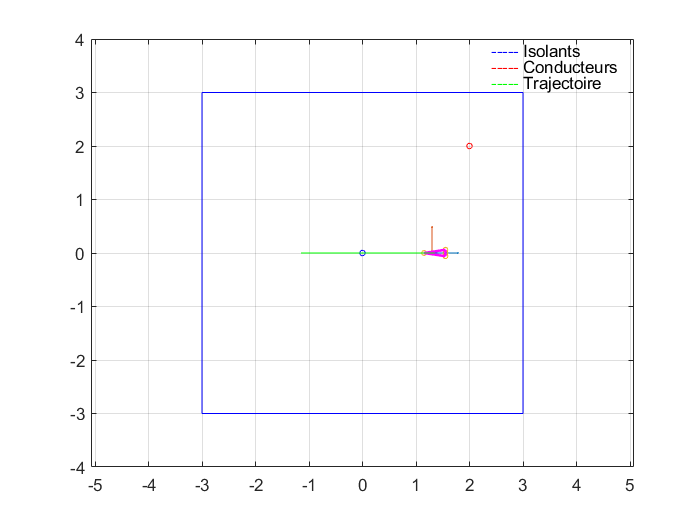
\includegraphics[width=0.5\textwidth]{assets/plot_currents/objet_isolant_2/objet_isolant_2_trajectoire.png}
    \caption{Représentation de l'aquarium pour la simulation. En bleu, les objets isolants (murs et objet), en rouge les objets conducteurs et en jaune la trajectoire suivi par le robot poisson.}
    \label{fig:objet_isolant_2_trajectoire}
\end{figure}
\begin{figure}[h!]
    \centering
    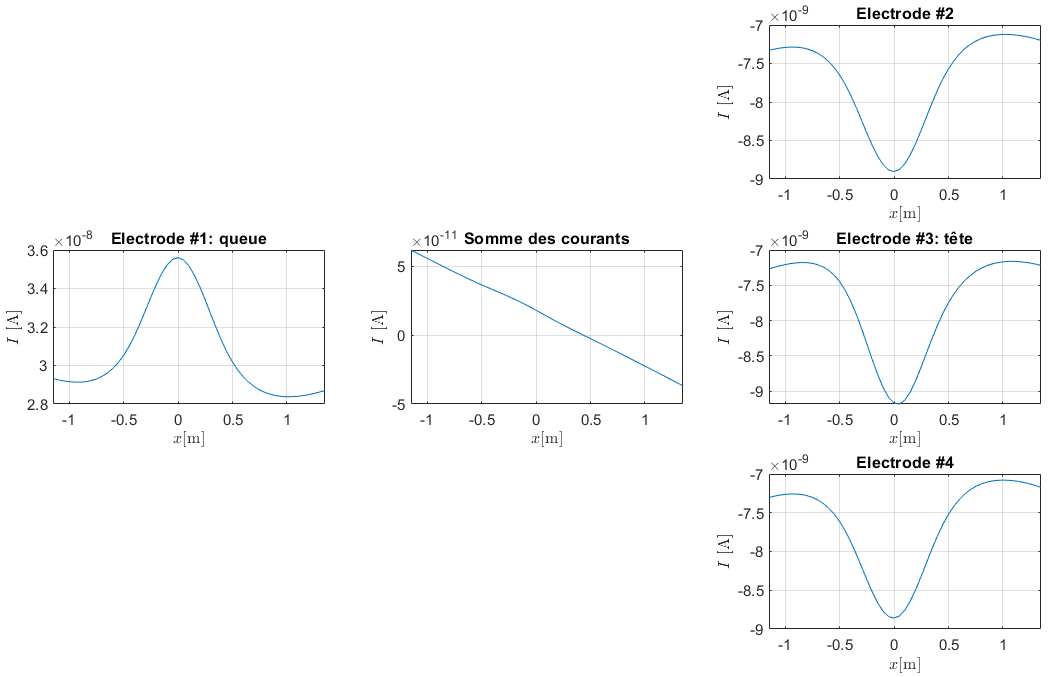
\includegraphics[width=0.9\textwidth]{assets/plot_currents/objet_isolant_2/objet_isolant_2.png}
    \caption{Courants obtenus dans l'électrode \#1 (queue), \#2, \#3 (tête) et \#4, lors de traverser un objet totalement isolant.}
    \label{fig:objet_isolant_2}
\end{figure}
\clearpage
\subsubsection{Cas d'un petit objet conducteur}
\begin{figure}[h!]
    \centering
    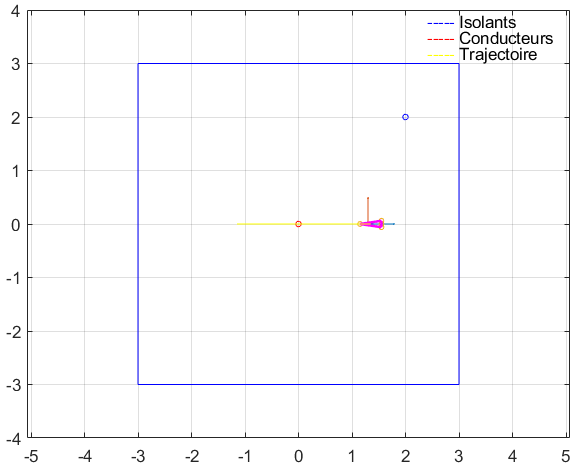
\includegraphics[width=0.5\textwidth]{assets/plot_currents/objet_conducteur_2/objet_conducteur_2_trajectoire.png}
    \caption{Représentation de l'aquarium pour la simulation. En bleu, les objets isolants (murs et objet), en rouge les objets conducteurs et en jaune la trajectoire suivi par le robot poisson.}
    \label{fig:objet_conducteur_2_trajectoire}
\end{figure}
\begin{figure}[h!]
    \centering
    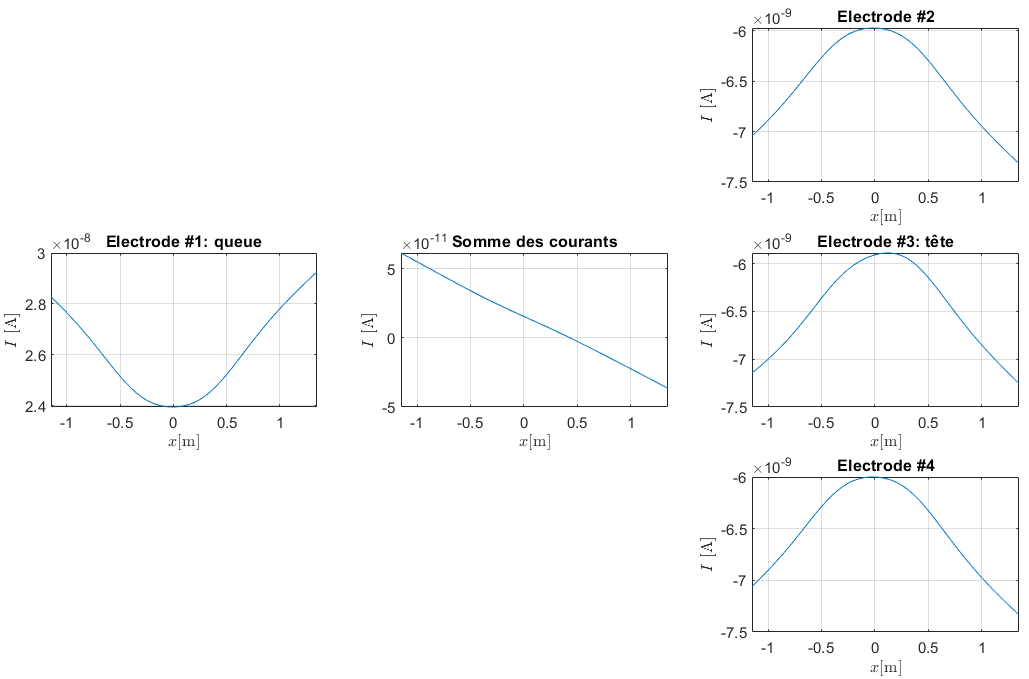
\includegraphics[width=0.9\textwidth]{assets/plot_currents/objet_conducteur_2/objet_conducteur_2.png}
    \caption{Courants obtenus dans l'électrode \#1 (queue), \#2, \#3 (tête) et \#4, lors de traverser un objet totalement conducteur.}
    \label{fig:objet_conducteur_2}
\end{figure}
\clearpage
\subsubsection{Cas d'un mur (isolant)}
\begin{figure}[h!]
    \centering
    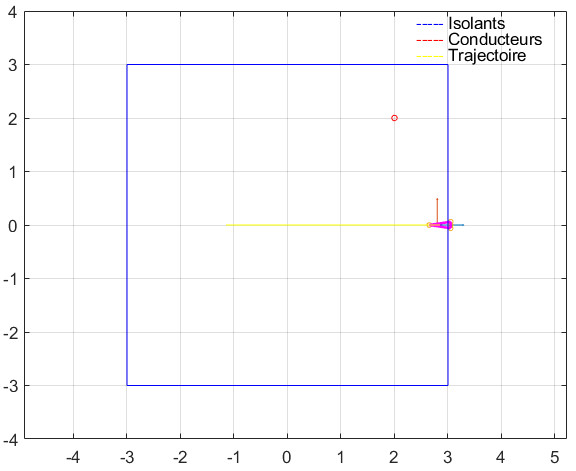
\includegraphics[width=0.5\textwidth]{assets/plot_currents/approximation_wall/approximation_wall_trajectoire.png}
    \caption{Représentation de l'aquarium pour la simulation. En bleu, les objets isolants (murs et objet), en rouge les objets conducteurs et en jaune la trajectoire suivi par le robot poisson.}
    \label{fig:approximation_wall_trajectoire}
\end{figure}
\begin{figure}[h!]
    \centering
    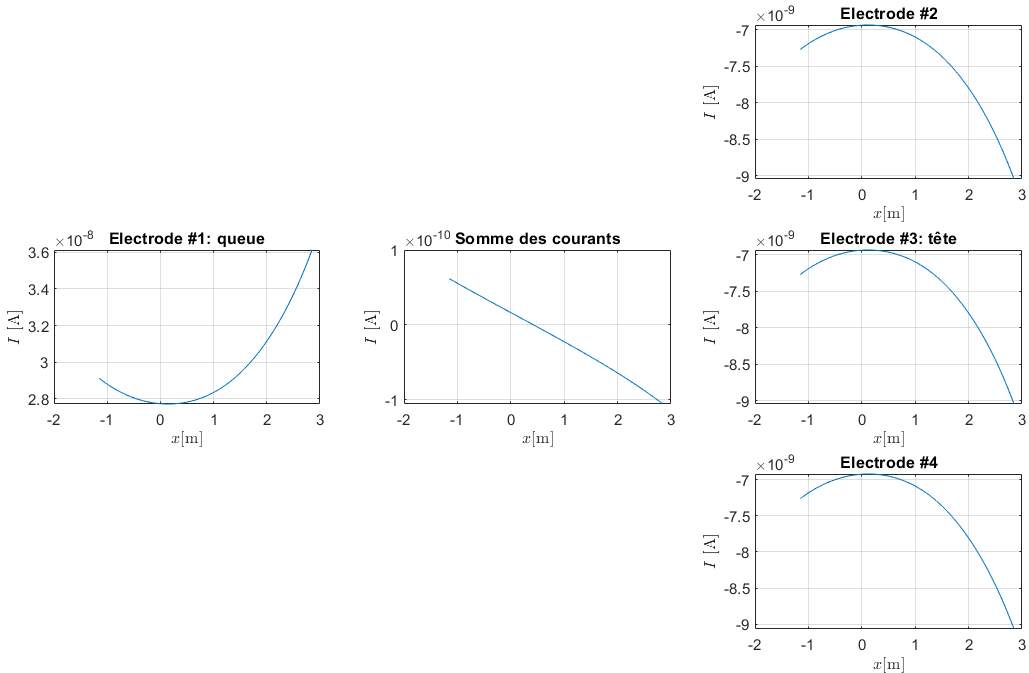
\includegraphics[width=0.9\textwidth]{assets/plot_currents/approximation_wall/approximation_wall.png}
    \caption{Courants obtenus dans l'électrode \#1 (queue), \#2, \#3 (tête) et \#4, lors de l'approximation à un mur.}
    \label{fig:approximation_wall}
\end{figure}
\section{Loi de commande} 
\subsection{Loi de contrôle et comportements} \label{sec:controle}
Afin d'étendre la stratégie bio-inspirée présentée précédemment au cas actif, nous considérons que les composantes perturbatrices $\delta \mathbf{I}$, en concret les scalaires axial $\delta I_{ax}$ et latéral $\delta I_{lat}$ présentés dans l'équation (\ref{eq:axial_lateral}).

La Table \ref{tab:proprietes} suggère d'appliquer la loi de contrôle suivante, d'après \cite{Boyer2013}: 

\begin{equation}
    v = C \quad ; \quad \omega = k \cdot \delta I_{lat}
\end{equation}
où $C$ est une constante positive qui permet au robot d'avancer vers l'avant, et $k$ est un gain pour contrôler la vitesse angulaire du robot poisson $\omega$. 

À partir de la Table \ref{tab:proprietes}, nous pouvons modifier le comportement dynamique du robot poisson: 
\begin{enumerate} [label=(\alph*), ref=(3.1.\alph*)]
    \item Si $k > 0$, cette loi de contrôle force \textbf{le capteur à être attiré par tout objet conducteur} et garantit que le capteur est repoussé par un objet isolant. \label{item:a}
    \begin{itemize}
        \item De ce fait, lorsqu'un objet conducteur conducteur se trouve à droite (ou à gauche, respectivement), le capteur se tourne vers la droite (ou la gauche, respectivement). Et lorsqu'un objet conducteur se trouve devant le capteur, le capteur avance sans changer d'orientation.
        \item En revanche, lorsqu'un objet isolant est situé à droite (ou à gauche, respectivement), cette loi de contrôle fait réagir le robot poisson comme s'il y avait un objet conducteur symétrique sur la gauche (ou sur la droite, respectivement).
    \end{itemize}
    \item \label{item:b} Si $k < 0$, cette loi force \textbf{le capteur à être attiré par tout objet isolant} et repoussé par les objets conducteurs. 
    \vspace{0.5cm}
    \item Si nous multiplions $k$ par le signe de $\delta I_{ax}$, nous obtenons les mêmes comportements pour des objets conducteurs ou isolants, ce qui assure au capteur, pour $k > 0$ d'être \textbf{attiré par tout objet}, et pour $k < 0$ d'être \textbf{repoussé par tout objet non transparent électriquement}. \label{item:c}
\end{enumerate}

\subsection{Résultats obtenus}

Personnellement, le cas \ref{item:a} ne marche pas très bien, mais les cas \ref{item:b} et \ref{item:c} marchent bien. 

Pour le cas \ref{item:b}, où $k < 0$, nous pouvons voir dans la Figure comment le robot poisson est attiré par l'objet isolant, indépendemment de ça position. 

%--------------------------------------- DEBUT DES ANNEXES --------------------------------------
\newpage
\begin{IMTAannexes}
	
%-------------------------------------------- ANNEXE 1  -----------------------------------------
\IMTAannexe{Exemple d'annexe}\label{sec:S_ANN_EX}

Un exemple d'annexe.
\section{Première partie}


\subsection{Sous-section}
\subsection{Sous-section}

\section{Deuxième partie}

\subsection{Sous-section}
\subsection{Sous-section}

%------------------------------------- -- FIN DES ANNEXES --------------------------------------
\end{IMTAannexes}

%-----------------------------------DEBUT DE LA BIBLIOGRAPHIE ----------------------------------
\newpage
%------------------ Ajout du renvoi vers la bibliographie dans le sommaire ---------------------
\phantomsection
\addcontentsline{toc}{section}{\refname}
%-----------------------------------------------------------------------------------------------

\begin{thebibliography}{99}
% \bibitem{[Lichtfouse2012]} Eric Lichtfouse, \emph{Rédiger pour être publié}, Springer, $2^{eme}$ édition, 2012 (cote bibliothèque IMT Atlantique Brest : $0.343$ LICH).
\bibitem{BENACHENHOU2014} Mohammed-Rédha BENACHENHOU, \emph{Électrolocation dans un contexte multi-robots: théorie et expérimentations}, Thèse de Doctorat, École Centrale de Nantes, 2014. 

\bibitem{Boyer2012} Frédéric Boyer, Pol Bernard Gossiaux, Brahim Jawad, Vincent Lebastard and Mathieu Porez, \emph{Model for a sensor inspired by electric fish}, JOURNAL OF IEEE TRANSACTIONS ON ROBOTICS, 2012.

\bibitem{Jackson2012} John David Jackson, \emph{Clasiccal Electrodynamics}, John Wiley \& Sons, 1962.

\bibitem{Boyer2013} Frédéric Boyer, Vincent Lebastard, Christine Chevallereau, and Noël Servagen, \emph{Underwater Reflex Navigation in Confined Environment Based on Electric Sense}, IEEE TRANSACTIONS ON ROBOTICS, VOL. 29, NO. 4, AUGUST 2013

\bibitem{BENACHENHOU} Mohammed-Rédha BENACHENHOU,  Frédéric Boyer, Christine Chevallereau, Vincent Lebastard, \emph{Fast simulator of the electric sense for complex scene}.

%----------------------------------- FIN DE LA BIBLIOGRAPHIE -----------------------------------
\end{thebibliography}
%---------------------------------------- Do not modify ----------------------------------------
\IMTAcoverpage
%------------------------------------ End of do not modify -------------------------------------

\end{document}

%***********************************************************************************************
%                                   FIN DU FICHIER D'EDITION
%***********************************************************************************************
